\graphicspath{ {Figures/blood_donation/} }

\chapter{Εθελοντική αιμοδοσία}\label{ch:Βlood Donations}

\section{Εθελοντική αιμοδοσία}
	Στο παρόν κεφάλαιο αναλύουμε τις βασικές έννοιες σχετικά με την αιμοδοσία οι οποίες εμπλέκονται στο θέμα της παρούσας διπλωματικής εργασίας.
	\subsection{Το αίμα}
	Το αίμα είναι το σπουδαιότερο βιολογικό υγρό του ανθρώπινου οργανισμού και αποτελεί ένα ανεκτίμητο προϊόν ζωής, το οποίο δεν μπορεί να κατασκευαστεί με συνθετικό τρόπο. Χωρίς της επαρκή ποσότητα αίματος, τα κύτταρα του ανθρώπινου σώματος δεν μπορούν να λάβουν το οξυγόνο και τα θρεπτικά συστατικά που τους είναι απαραίτητα για να επιβιώσουν \cite{aboutBlood}. Επιπλέον το σώμα δεν θα μπορούσε να αντιμετωπίσει βλαπτικούς παράγοντες, να αποβάλει τοξικά προϊόντα και να ρυθμίσει τις παραμέτρους του εσωτερικού του περιβάλλοντος \cite{circulatorySystem}. Αν και η τεράστια αξία και χρησιμότητα του αίματος είναι αδιαμφισβήτητη η ύπαρξη αρκετών εθελοντικών αιμοδοσιών για να καλυφθούν οι ανάγκες για αίμα αποτελεί μείζων πρόβλημα.
	
	Το αίμα αποτελείται από ερυθρά αιμοσφαίρια, λευκά αιμοσφαίρια, αιμοπετάλια τα οποία εναιωρούνται μέσα στο πλάσμα και πρωτεΐνες. Στο σχήμα \ref{fig:basic_blood_diagram}  παρακάτω παρουσιάζονται τα διάφορα συστατικά από τα οποία αποτελείται το αίμα:
	\begin{figure}[h]
	    \centering
	    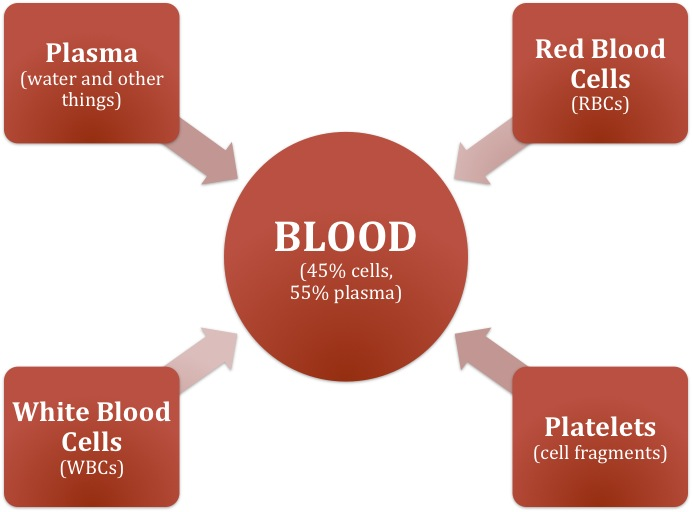
\includegraphics[width=0.7\textwidth]{basic_blood_diagram.jpg}
	    \caption{Συστατικά του αίματος}
	    \label{fig:basic_blood_diagram}
	\end{figure}
	 
	Το πλάσμα αποτελεί το μεγαλύτερο και κύριο συστατικό του αίματος, καταλαμβάνοντας το 55\% του συνολικού όγκου του. Είναι ένα υποκίτρινο υγρό μέσω του οποίου μεταφέρονται αιμοσφαίρια, πρωτεΐνες και άλλες ουσίες. Αποτελείται κατά 91,5\% από νερό, κατά 7\% από πρωτεΐνες, όπως η λευκωματίνη (αλβουμίνη), οι σφαιρίνες και το ινωδογόνο, και κατά 1,5\% από άλλες ουσίες, όπως θρεπτικά συστατικά, ορμόνες, αναπνευστικά αέρια, ηλεκτρολύτες, βιταμίνες και άχρηστες αζωτούχες ουσίες \cite{bloodPlasma}. Η κύρια λειτουργία που επιτελεί είναι η μεταφορά υγρών και υδατοδιάλυτων ουσιών όπως είναι οι ορμόνες και βασικές .

	Το υπόλοιπο 45\% του αίματος αποτελείται από αιμοσφαίρια και κυρίως ερυθρά αιμοσφαίρια, λευκά αιμοσφαίρια και αιμοπετάλια. Τα ερυθρά αιμοσφαίρια είναι τα πιο πολυάριθμα κύτταρα σε κυκλοφορία και δίνουν στο αίμα το χαρακτηριστικό κόκκινο χρώμα του. Τα ερυθρά αιμοσφαίρια χρησιμοποιούνται ευρέως, για να αναπληρώνουν την απώλεια αίματος που προκαλείται από αιμορραγία κατά τη γέννα, κατά τη διάρκεια χειρουργικής επέμβασης και κατά τη διάρκεια ατυχημάτων. Η μετάγγιση ερυθρών αιμοσφαιρίων μπορεί επίσης να είναι σωτήρια για τη ζωή του ασθενούς σε συγκεκριμένους τύπους αναιμίας. Η λειτουργία τους αφορά τη διατήρηση των ιστών στη ζωή καθώς μεταφέρουν σε αυτούς οξυγόνο και απομακρύνουν το διοξείδιο του άνθρακα. Η εκατοστιαία αναλογία ερυθρών αιμοσφαιρίων ανά μονάδα όγκου αίματος ονομάζεται αιματοκρίτης \cite{hematologyBasics}.
	
	Τα λευκά αιμοσφαίρια ή λευκοκύτταρα (WBC) αποτελούν λιγότερο από το 1\% του ολικού αίματος. Η πρωταρχική λειτουργία των λευκοκυττάρων είναι η καταπολέμηση των λοιμώξεων μέσω της επίθεσης και της καταστροφής επιβλαβών ξένων ουσιών. Σχηματίζονται στο μυελό των οστών, στη σπλήνα και τους λεμφαδένες \cite{whiteBloodCells}.
	
	Τα αιμοπετάλια ή θρομβοκύτταρα παράγονται από το μυελό των οστών και αποτελούν λιγότερο από το 1\% του πλήρους αίματος. Παίζουν καθοριστικό ρόλο στην πήξη του αίματος και την αιμόσταση, δηλαδή στην αναστολή της αιμορραγίας ή της κυκλοφορίας. Σχηματίζουν θρόμβους ώστε να αποτρέπεται η διαρροή αίματος από τις πληγές και αν ο αριθμός τους είναι χαμηλός, αυτό μπορεί να οδηγήσει σε εύκολη δημιουργία μωλώπων και σε μεγάλη αιμορραγία. Οι ασθενείς που έχουν λευχαιμία ή ανεπάρκεια μυελού των οστών, συνήθως έχουν χαμηλό ποσοστό αιμοπεταλίων και χρειάζονται αιμοπετάλια, για να διαφυλάξουν τη λειτουργία της πήξης του αίματός τους \cite{hematologyBasics}.
	
	Στο σχήμα \ref{fig:blood_cells_characteristics} βλέπουμε μια σύνοψη των βασικών χαρακτηριστικών των συστατικών του αίματος.
\begin{figure}[H]
	    \centering
	    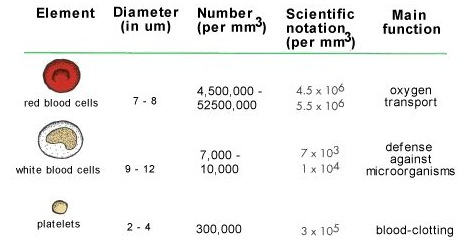
\includegraphics[width=0.7\textwidth]{blood_cells_characteristics.jpg}
	    \caption{Χαρακτηριστικά των κυττάρων του αίματος}
	    \label{fig:blood_cells_characteristics}
\end{figure}

	Τα κύτταρα του αίματος ανανεώνονται συνεχώς, όπως φαίνεται από τη διάρκεια ζωής στο αίμα των ερυθρών αιμοσφαιρίων (120 ημέρες), των αιμοπεταλίων (10 ημέρες) και των κοκκιοκυττάρων (9 ώρες). Ο χρόνος ζωής των λεμφοκυττάρων (Τ και Β κυττάρων) ποικίλλει εξαιρετικά από ώρες έως χρόνια. Η παραγωγή ενεργών κυττάρων του αίματος λαμβάνει χώρα κατά κύριο λόγο στο μυελό των οστών. Ωστόσο ο σπλήνας, οι λεμφαδένες και οι βοηθητικοί λεμφοειδείς ιστοί είναι επίσης θέσεις συνεχιζόμενης παραγωγής κυττάρων, κυρίως λεμφικής σειράς \cite{textbookOfMedicine}.
	
	Ένας υγιής ενήλικας έχει περίπου 5-6 λίτρα αίματος \cite{bloodVolume}, και μπορεί να υποστεί απώλεια 500 ml χωρίς να υποστεί προβλήματα υγείας και να χρειαστεί κάποια μετάγγιση αίματος. Βέβαια άμα υποστεί απώλεια της τάξης των 1000-1500 ml σε μικρό χρονικό διάστημα ή κάποια συστατικά του αίματος (αιμοπετάλια, ερυθρά αιμοσφαίρια) είναι κάτω από τα απαιτούμενα επίπεδα λόγω ασθένειας (καρκίνος, αναιμία κτλπ) ή λόγω κάποιας εγχείρησης, τότε χρειάζεται μετάγγιση αίματος \cite{Stainsby01092000}.
		\subsubsection{Ομάδες αίματος και συμβατότητα}	
			Στην επιφάνεια του ερυθρού αιμοσφαιρίου υπάρχουν διάφορα αντιγόνα ή ουσίες των ομάδων αίματος (blood group substances). Σήμερα είναι γνωστά 23 συστήματα ομάδων αίματος, γενετικά ανεξάρτητα το ένα από το άλλο. Κληρονομούνται σύμφωνα με τους νόμους του Mendel και η γνώση τους είναι εξαιρετικά χρήσιμη στην Ιατροδικαστική (έλεγχος πατρότητας), σε ανθρωπολογικές μελέτες αλλά κυρίως για τη σωστή και ασφαλή μετάγγιση αίματος στην κλινική πράξη \cite{dawkins}. Κάθε σύστημα ομάδων αίματος περιλαμβάνει μία σειρά αντιγόνων που σχετίζονται ως προς τη δομή. Συνολικά, τα συστήματα αυτά περιλαμβάνουν περισσότερα από 400 αντιγόνα. Οι ουσίες των ομάδων αίματος δεν περιορίζονται μόνο στη μεμβράνη των ερυθρών αιμοσφαιρίων αλλά βρίσκονται ακόμη σε κύτταρα πολλών ιστών καθώς και σε υγρά του σώματος, όπως σάλιο, γαστρικό υγρό, σπέρμα, ούρα, και γάλα. Τα συστήματα ομάδας αίματος συμπεριλαμβάνουν τα ΑΒΟ, τα Rh, MNS, Kell, Duffy, Kidd και άλλα.
			
			Το πιο γνωστό και πιο ευρείας χρήσης είναι το σύστημα ΑΒΟ. Είναι το πρώτο σύστημα που ανακαλύφθηκε το 1900 από τον Landsteiner (Βραβείο Νομπέλ Ιατρικής 1930) \cite{landsteinerABO}. Η ανακάλυψη αυτή άνοιξε το δρόμο για την ασφαλή μετάγγιση αίματος. Το σύστημα ΑΒΟ εξακολουθεί και σήμερα να είναι το πιο σημαντικό στη μετάγγιση. Το σύστημα συνδέεται με τρία αντιγόνα Α, Β και Η. Το σύστημα χαρακτηρίζεται από την παρουσία ή την απουσία στα ερυθρά αιμοσφαίρια των αντιγόνων (συγκολλητινογόνων). Με συνδυασμό αυτών διακρίνονται τέσσερις ομάδες αίματος, η ΑΒ, η Α, η Β, και η Ο. Η ομάδα ΑΒ χαρακτηρίζεται από την παρουσία στα ερυθρά αιμοσφαίρια και των δύο αντιγόνων Α και Β. Η ομάδα Α χαρακτηρίζεται από την παρουσία του αντιγόνου Α. Η ομάδα Β χαρακτηρίζεται από την παρουσία του αντιγόνου Β. Τέλος η ομάδα Ο δεν περιέχει κανένα από τα αντιγόνα Α ή Β, αλλά περιέχει το αντιγόνο Η. Το τελευταίο υπάρχει σε όλες τις ομάδες αλλά ιδιαιτέρως παρατηρείται στην ομάδα Ο.
			
			Στον ορό του αίματος των διαφόρων ατόμων παρατηρούνται φυσιολογικές συγκολλητίνες ομόλογοι των συγκολλητινογόνων Α και Β. Οι φυσιολογικές συγκολλητίνες είναι οι α (anti- A) και οι β (anti-B). Στον ορό δεν υπάρχει ποτέ η συγκολλητίνη η ομόλογος προς το συγκολλητινογόνο που υπάρχει στα ερυθρά αιμοσφαίρια του ιδίου ατόμου. Έτσι στον ορό του αίματος ΑΒ δεν υπάρχει καμία συγκολλητίνη. Στον ορό της ομάδας Α υπάρχει η συγκολλητίνη anti-B ή β. Στον ορό της ομάδας Β υπάρχει η συγκολλητίνη anti-Α ή α. Τέλος στον ορό της ομάδας Ο υπάρχουν και οι δύο συγκολλητίνες α και β. Η συγκολλητίνη α αντιδρά με το συγκολλητινιγόνο Α και η συγκολλητίνη β αντιδρά με το συγκολλητινιγόνο Β. Εάν επομένως σε μία μετάγγιση αίματος ο ορός του ασθενούς (δέκτη) έχει συγκολλητίνες (α ή β, α και β), τότε αυτές θα συγκολλήσουν τα ερυθρά αιμοσφαίρια του δότη, όταν στα αιμοσφαίρια αυτά υπάρχουν συγκολλητινογόνα Α ή Β ή Α και Β. Στην περίπτωση αυτή τα συγκολλημένα ερυθρά αιμοσφαίρια μπορεί να προκαλέσουν ακόμη και το θάνατο του δέκτη. Στο σχήμα \ref{fig:blood_antibodies_antigons} φαίνονται συγκεντρωτικά τα στοιχεία που αναλύσαμε παραπάνω.		
	\begin{figure}[h!]
	    \centering
	    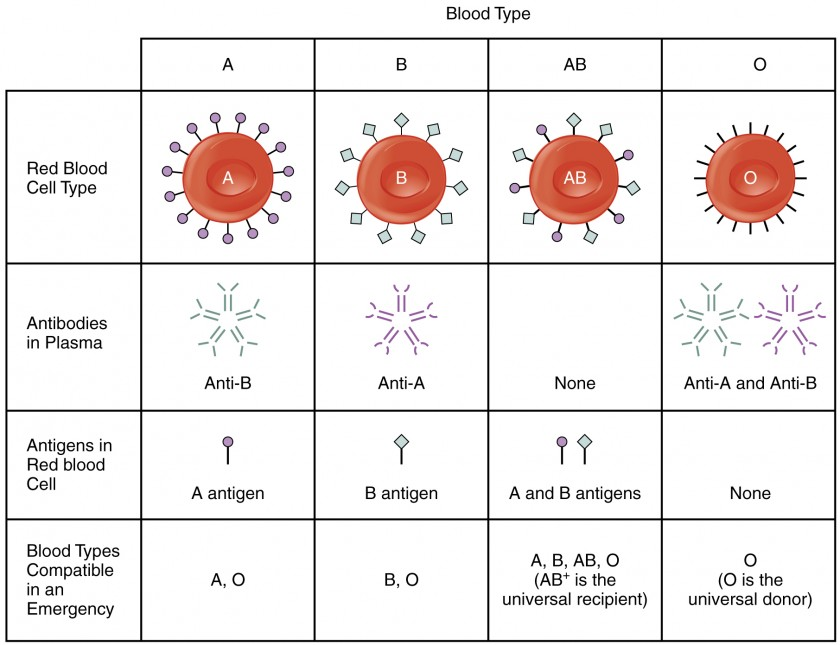
\includegraphics[width=0.7\textwidth]{blood_antibodies_antigons.jpg}
	    \caption{Αντισώματα και αντιγόνα του αίματος}
	    \label{fig:blood_antibodies_antigons}
	\end{figure}
			
			Στις μεταγγίσεις πρέπει να λαμβάνεται υπόψη και ένας άλλος
παράγοντας, που λέγεται παράγοντας Rhesus, επειδή ανακαλύφθηκε πρώτα στα ερυθρά
αιμοσφαίρια του πιθήκου Rhesus Maccacus. Το σύστημα Rhesus είναι το δεύτερο κατά
σπουδαιότητα σύστημα ομάδων αίματος μετά το ΑΒΟ. Η γνώση του είναι απαραίτητη για
την ασφαλή μετάγγιση αίματος, ενώ είναι το σύστημα, που κυρίως ευθύνεται για την
αιμολυτική νόσο του νεογνού. Σήμερα είναι γνωστά περί τα 50 αντιγόνα που ανήκουν στο
σύστημα Rhesus. Από αυτά τα πέντε είναι τα κύρια και βασικά. Το κυριότερο αντιγόνο είναι
το D και άτομα που το έχουν στα ερυθρά αιμοσφαίρια είναι Rh-Θετικά ή Rh (+), ενώ αυτά
που δεν το έχουν είναι Rh-Αρνητικά ή Rh (-). Το αντιγόνο D είναι εξαιρετικά ανοσογόνο
(immunogenic) και άτομα Rh-Αρνητικά, όταν εκτεθούν σε αυτό, μπορούν να σχηματίσουν
anti-D αντισώματα. Το 85\% των λευκών ανθρώπων έχουν τον παράγοντα αυτό, δηλαδή είναι
Rh-Θετικοί και το 15\% δεν το έχουν, δηλαδή είναι Rh-Αρνητικοί \cite{Landsteiner01011940}. 

Συμβάντα μπορεί να παρατηρηθούν, αν δεν προσδιοριστεί ο παράγοντας Rhesus, στις εξής
περιπτώσεις.
\begin{enumerate}
	\item Σε άτομα στα οποία έγινε μια πρώτη μετάγγιση και στα οποία μια δεύτερη μετάγγιση μπορεί να είναι θανατηφόρα
	\item Στις γυναίκες στις οποίες γίνεται μετάγγιση κατά τη διάρκεια της εγκυμοσύνης τους
	\item Στις γυναίκες που γέννησαν ήδη το πρώτο τους παιδί και στις οποίες μετά από λίγο γίνεται μετάγγιση
	\item Στα έμβρυα λόγω του παράγοντα Ρέζους μπορεί να προκληθεί μια πολύ σοβαρή πάθηση που λέγεται ερυθροβλάστωση των εμβρύων (αν η μητέρα είναι Ρέζους αρνητική, ο πατέρας Ρέζους θετικός και το έμβρυο επίσης Ρέζους θετικό). Κατά την αρρώστια αυτή τα αιμοσφαίρια του εμβρύου συγκολλούνται και προκαλείται τελικά ο θάνατος του. Μπορεί να σωθεί μόνο, αν γεννηθεί ζωντανό και γίνει αλλαγή του αίματος του (αφαιμαξομετάγγιση) με άλλο αίμα Ρέζους αρνητικό
\end{enumerate}

Βάση όσων έχουν αναφερθεί παραπάνω, στο σχήμα \ref{fig:blood_compatibility} βλέπουμε την συμβατότητα των διάφορων συνδυασμών.
	\begin{figure}[h!]
	    \centering
	    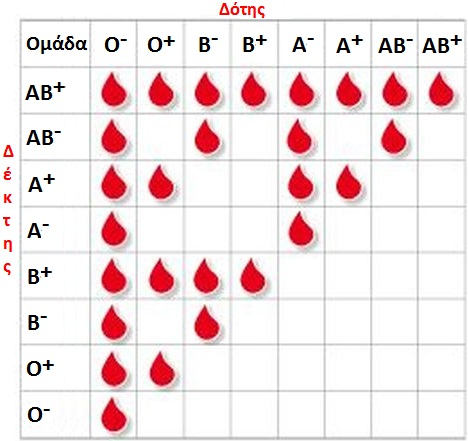
\includegraphics[width=0.5\textwidth]{blood_compatibility.jpg}
	    \caption{Συμβατότητα ομάδων αίματος}
	    \label{fig:blood_compatibility}
	\end{figure}
	
	Από την άλλη μεριά η μετάγγιση πλάσματος έχει τους αντίθετους κανόνες αφού τα αντιγόνα βρίσκονται στο πλάσμα. Για παράδειγμα ένας ασθενής με τύπο αίματος O μπορεί να λάβει πλάσμα από τις ομάδες αίματος A,B και ΑΒ αφού το πλάσμα του τύπου Ο περιέχει αντιγόνα και της Α και της Β. Στον πίνακα \ref{tab:plasma_compatibility} βλέπουμε τη συμβατότητα πλάσματος των διάφορων συνδυασμών.
\begin{table}[H]
	\centering
	\begin{tabular}{l|llll}
		Ασθενής & \multicolumn{4}{l}{Αιμοδότης} \\ \hline
			& Ο     & Α     & Β     & ΑΒ    \\
		Ο       & Ναι   & Ναι   & Ναι   & Ναι   \\
		Α       & Όχι   & Ναι   & Όχι   & Ναι   \\ 
		Β       & Όχι   & Όχι   & Ναι   & Ναι   \\
		ΑΒ      & Όχι   & Όχι   & Όχι   & Ναι  
	\end{tabular}
	\caption{Συμβατότητα πλάσματος}
	\label{tab:plasma_compatibility}
\end{table}
	Σε αυτό το σημείο θα πρέπει να αναφερθεί ότι η κατανομή του πληθυσμού στις διάφορες ομάδες αίματος δεν είναι ισόποση. Στο σχήμα \ref{fig:blood_distribution} βλέπουμε την κατανομή σε επιλεγμένες χώρες.
\begin{figure}[h!]
	    \centering
	    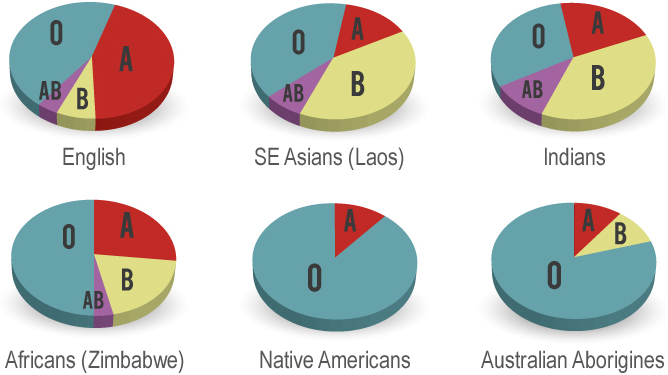
\includegraphics[width=0.7\textwidth]{blood_distribution.jpg}
	    \caption{Κατανομή ομάδων αίματος}
	    \label{fig:blood_distribution}
\end{figure}	

	\subsection{Αιμοδοσία}
	Με τον όρο αιμοδοσία εννοούμε τη χορήγηση αίματος από υγιείς δότες σε άτομα στα
οποία η κατάσταση της υγείας τους απαιτεί μετάγγιση. Κατ' επέκταση με τον όρο αιμοδοσία εννοούμε την όλη οργάνωση που ασχολείται με τη λήψη, επεξεργασία, συντήρηση και διάθεση του αίματος και των Παραγώγων του \cite{bloodDonationDefinition}. Η αιμοδοσία καλείται εθελοντική, επειδή αφορά σε πράξη που εκτελεί κάποιος με τη θέλησή του και με μοναδικά κίνητρα αισθήματα αλληλεγγύης και αλτρουισμού \cite{1973}. 

Ως επιστημονικός τομέας, η αιμοδοσία αποτελεί ιδιαίτερο κλάδο της αιματολογίας με τεράστια ανάπτυξη τα τελευταία 20 χρόνια. Η ανάπτυξη της αιμοδοσίας ως εξειδικευμένου τομέα, καθώς και η αλματώδης ανάπτυξή της, οδήγησαν στην ανάγκη να πλαισιώνεται από ιατρικό, νοσηλευτικό και τεχνικό προσωπικό υψηλής στάθμης με εξειδίκευση στον τομέα της
αιμοδοσίας.  
	
	Η μετάγγιση αίματος γίνεται τακτικά σε εγχειρήσεις, τραυματίες, γαστρορραγίες και σε τοκετούς για την αναπλήρωση της απώλειας σημαντικής ποσότητας αίματος. Στις περισσότερες περιπτώσεις η μετάγγιση αίματος χρησιμοποιείται ως προσωρινή μορφή θεραπείας. Σε αυτές τις περιπτώσεις ο ασθενής χρειάζεται αρκετές μονάδες αίματος αλλά μόλις η κατάσταση του θεωρηθεί εκτός κινδύνου, δεν χρειάζεται περεταίρω μετάγγιση αίματος. Βέβαια, υπάρχουν και περιπτώσεις όπου ο ασθενής χρειάζεται μεταγγίσεις αίματος εφόρου ζωής. Μερικές ευρέως γνωστές ασθένειες που απαιτούν κάτι τέτοιο είναι η Β-Θαλασσαιμία (η Ελλάδα έχει τα υψηλότερα ποσοστά), αιμοφιλία και λευχαιμία \cite{thalassaemiaLongTerm}.

	Αν και υπάρχουν κάποιες περιπτώσεις οι οποίες απαιτούν μετάγγιση ολικού αίματος, η πλειονότητα του αίματος διασπάται μετά την δωρεά και τα απαιτούμενα προϊόντα αίματος μεταφέρονται στον ασθενή. Ακολουθώντας την παραπάνω προσέγγιση, από την μία μεριά ο ασθενής δεν λαμβάνει περιττά συστατικά και από την άλλη μεριά από μία μονάδα ολικού αίματος μπορούν να επωφεληθούν περισσότερα του ενός ατόμου. Η διάρκεια ζωής των διάφορων συστατικών του αίματος φαίνονται στον πίνακα \ref{tab:blood-shelf-life} παρακάτω \cite{Basu2014}:
	
\begin{table}[H]
		\centering
		\begin{tabular}{l|ll}
			\hline
			Συστατικό          & Διάρκεια  & Θερμοκρασία \\ \hline
			Ολικό αίμα         & 24 ώρες   & 20-24       \\
			Ερυθρά αιμσοφαίρια & 42 μέρες  & 4           \\
			Αιμοπετάλια        & 3-5 μέρες & 20-24       \\
			Πλάσμα             & 1 χρόνος  & -18        
		\end{tabular}
		\caption{Διάρκεια ζωής συστατικών αίματος}
		\label{tab:blood-shelf-life}
\end{table}	

Από τα δεδομένα του παραπάνω πίνακα γίνεται εύκολα εμφανές ότι είναι προτιμότερο να αποθηκευόνται τα συστατικά του αίματος πάρα το ολικό αίμα, ενώ παράλληλα γίνεται εμφανής η ανάγκη για συνεχή παροχή αιμοδοσιών.
	
	 Το αίμα που χρησιμοποιείται στις μεταγγίσεις πρέπει να προέρχεται από υγιή άτομα. Το αίμα δεν είναι μόνο ζωντανός ιστός, αλλά έχει επιπλέον την ιδιότητα να ανανεώνεται και τα υγιή άτομα διαθέτουν μηχανισμούς αύξησης της παραγωγής αίματος. Έτσι με την αιμοδοσία προσφέρεται εύκολα το δώρο της ζωής χωρίς το φόβο ότι η τακτική αιμοδοσία θα προκαλέσει εξασθένηση του οργανισμού και θα οδηγήσει σε αδυναμία η επιτάχυνση της γήρανσης.
	 
	Στόχος είναι οι εθελοντές, που πληρούν τα κριτήρια για αιμοδοσία να γίνονται τακτικοί αιμοδότες, δηλαδή να πραγματοποιούν δωρεά αίματος αρκετές φορές το χρόνο και να παραμένουν στον κατάλογο των ενεργών αιμοδοτών για πολλά χρόνια. Η διατήρηση ενός υψηλού επιπέδου ποιότητας παρεχόμενων υπηρεσιών στην υπηρεσία αιμοδοσίας συνίσταται στην προτεραιότητα ικανοποίησης των αναγκών και των προσδοκιών των εθελοντών αιμοδοτών. Ωστόσο είναι σημαντικό να επισημάνουμε ότι μια επένδυση στην προσέλκυση και την διατήρηση εθελοντών, δεν θα αποδώσει μόνο ασφαλή αποθέματα αίματος και προστασία της υγείας τόσο στον δότη όσο και στον λήπτη, αλλά και σημαντική εξοικονόμηση κόστους για την υπηρεσία μέσω της μείωσης του αριθμού μονάδων αίματος που πρέπει να απορριφθούν λόγω της ανεύρεσης θετικών δεικτών λοιμωδών νοσημάτων. 
	
	Επιπλέον η προσέλκυση και η διατήρηση των εθελοντών αιμοδοτών είναι μια δυναμική λειτουργία που σχεδιάζεται κάθε φορά ανάλογα με την μελέτη και ανάλυση των παραμέτρων της συγκεκριμένης κοινωνικής ομάδας που απευθυνόμαστε σε σχέση με την αξιολόγηση και εκτίμηση των αναγκών σε αίμα και την υπάρχουσα κατάσταση στο χώρο της.
		\subsubsection{Διαδικασία της Αιμοδοσίας}
		 Η διαδικασία της αιμοδοσίας είναι lorem ipsum dolor lorem ipsum dolor
	\subsection{Εθελοντές αιμοδότες}
		\subsubsection{Κριτήρια επιλογής αιμοδοτών} 
			Βασικός στόχος και υποχρέωση των υπηρεσιών μετάγγισης αίματος είναι να συλλέξουν αίμα από υγιείς αιμοδότες, ώστε αφενός να προφυλαχθεί η δική τους υγεία και αφετέρου να προστατευθεί ο αιμολήπτης ασθενής από τη μετάδοση ασθενειών ή φαρμακευτικών ουσιών που μπορεί δυνητικά να είναι βλαβερά για την υγεία του. Ο υποψήφιος αιμοδότης κατά τη λήψη του ιστορικού πρέπει να αναφέρει τυχόν συμπτώματα, ώστε να βοηθήσει το ιατρικό προσωπικό να κρίνει με ασφάλεια την πιθανότητα κινδύνου. Κάθε πρόβλημα υγείας που ενδεχομένως έχει ο υποψήφιος αιμοδότης, πρέπει να συζητείται με τον υπεύθυνο γιατρό της αιμοδοσίας, ο οποίος και κρίνει τελικά για τη καταλληλότητα της αιμοληψίας. Η διαδικασία θα πρέπει να είναι τέτοια έτσι ώστε και να εξασφαλίζεται ασφαλή αιμοδοσία και παροχή αίματος αλλά και να μην απορρίπτονται υγιείς αιμοδότες οι οποίοι θα μπορούσαν να συνεισφέρουν \cite{bloodDonorSelection}.
			
			Ο αιμοδότης πρέπει να είναι σε καλή υγεία και απαλλαγμένος από μεταδοτικές ασθένειες. Όμως κάθε άνθρωπος είναι επιρρεπής σε μικρο-αδιαθεσίες. Αυτές είναι πόνοι κάθε είδους, ακμή, πονόλαιμοι και δυσπεψία. Όλα αυτά δεν αποτελούν στοιχεία απόρριψης του αιμοδότη. Εάν ο δότης υποβάλλεται σε φαρμακευτική αγωγή ή έχει υποβληθεί στο άμεσο παρελθόν, πρέπει να σημειωθούν τα παρακάτω σχετικά με τα φάρμακα που παίρνει. Η ποσότητα του φαρμάκου, δηλαδή η πυκνότητα του φαρμάκου στον οργανισμό του δότη και η ταχύτητα απορρόφησης ή η αποβολή του. Το φάρμακο μπορεί να έχει δυσμενή επίπτωση στο δέκτη εφόσον η περιεκτικότητα του φαρμάκου στο δότη είναι αυξημένη. Εάν ο δέκτης είναι αλλεργικός σ' αυτό το φάρμακο ή εάν ο δέκτης είναι έγκυος γυναίκα μπορεί να προκληθεί μέχρι και τερατογένεση. Το φάρμακο μπορεί να διαταράξει το αίμα του δότη, π.χ. τη λειτουργικότητα των αιμοπεταλίων. Παρόλο ότι τα φαινόμενα αυτά έχουν αναγνωριστεί, η συχνότητά τους δεν μελετήθηκε ακόμη καλά. Εάν λοιπόν ο αιμοδότης λαμβάνει φάρμακα, δεν σημαίνει ότι αναγκαστικά δεν μπορεί να προσφέρει αίμα. Σε κάθε περίπτωση όμως είναι ορθό να ενημερώνεται ο γιατρός και το προσωπικό για τα φάρμακα που λαμβάνει και ανάλογα θα κριθεί εάν μπορεί να προσφέρει αίμα \cite{bloodDonorSelection}. 
			
		Υπάρχουν καταστάσεις και νοσήματα που αποκλείουν δια παντός την αιμοδοσία, όπως είναι το AIDS, οι ηπατίτιδες, η ελονοσία, η χρήση ενδοφλεβίων ναρκωτικών, οι κακοήθειες, η υπέρταση, ο σακχαρώδης διαβήτης ή σοβαρά χρόνια νοσήματα. Στις περισσότερες περιπτώσεις, όμως, ο αποκλεισμός είναι μόνο πρόσκαιρος.  Ο αποκλεισμός αυτός γίνεται για να μην επιβαρυνθεί η υγεία του αιμοδότη και για να διασφαλιστεί η ποιότητα του αίματος που θα μεταγγιστεί στο λήπτη. Μελέτες έχουν δείξει ότι ο προσωρινός αποκλεισμός από την αιμοδοσία έχει έντονο αρνητικό αντίκτυπο στην μελλοντική επιστροφή του αιμοδότη \cite{Custer2011}\cite{Custer2007}. Για αυτό είναι υψίστης σημασίας να δίνονται ξεκάθαρα διαστήματα αποκλεισμού και να ενθαρρύνονται οι εθελοντές να επιστρέψουν μετά το πέρας αυτού του διαστήματος. Στο σύστημα που προτείνουμε στη παρόν διπλωματική έχει γίνει μέριμνα για τέτοιες περιπτώσεις και προτείνετε ένα σύστημα κατάλληλων ειδοποιήσεων.
		
		Η καλή επικοινωνία μεταξύ του αιμοδότη και του προσωπικού της αιμοδοσίας διατηρεί τη σχέση εμπιστοσύνης και διασφαλίζει την καλή ποιότητα του αίματος που παρέχεται στους ασθενείς που χρειάζονται αίμα και τα παράγωγά του. Αίμα μπορούν να δώσουν όλοι οι υγιείς άντρες και γυναίκες ηλικίας 18 - 62 ετών, κάθε 3 - 4 μήνες. 
		\subsubsection{Κατηγορίες αιμοδοτών}
			Οι αιμοδότες μπορούν να χωριστούν σε τρεις μεγάλες κατηγορίες:
\begin{enumerate}
	\item Οι εθελοντές αιμοδότες (Volunteer Donors - VDs) οι οποίοι αιμοδοτούν με δική τους πρωτοβουλία καθαρά για ανθρωπιστικούς λόγους, χωρίς να λαμβάνουν κάποιο οικονομικό αντάλλαγμα ή οτιδήποτε που θα μπορούσε να θεωρηθεί ως αντικαταστατό του χρήματος.
	\item Οι δότες αντικατάστασης (Replacement Donors - RDs), οι οποίοι αιμοδοτούν προκειμένου να καλύψουν τις ανάγκες που προκύπτουν από συγγενείς ή φίλους οι οποίοι νοσηλεύονται.
	\item Δότες αίματος επί πληρωμή οι οποίοι λαμβάνουν πληρωμή από την οικογένεια η οποία δεν μπορεί να παρέχει η ιδία δότη αντικατάστασης για το συγγενικό τους πρόσωπο.
\end{enumerate} 

Σε αυτό το σημείο ότι η τρίτη κατηγορία αιμοδοτών εμφανίζεται μόνο σε τριτοκοσμικές χώρες και κυρίως σε χώρες της Αφρικής. Στατιστικά στοιχεία έχουν δείξει ότι οι τακτικοί εθελοντές αιμοδότες (VDs) σχετίζονται με ασφαλέστερες παροχές αίματος σε σχέση με τους δότες αντικατάστασης όσον αφορά τις μεταδιδόμενες κατά την μετάγγιση ασθένειες \cite{Liu1998}.

Στοιχεία του Παγκόσμιου Οργανισμού Υγείας (WHO) και του Συμβουλίου της Ευρώπης υποδεικνύουν ότι το αίμα και τα παράγωγα του αίματος θα πρέπει να συλλέγονται αποκλειστικά από τακτικούς μη αμειβόμενους εθελοντές \cite{VOX:VOX5295}. Τα συστήματα αιμοδοσίας τα οποία στηρίζονται στους εθελοντές αιμοδότες οι οποίοι δίνουν αίμα σε σταθερή βάση, έχουν τη δυνατότητα να διαχειριστούν καλύτερα τις παροχές αίματος και να προγραμματίσουν τις μεταγγίσεις, επιταχύνοντας την όλη διαδικασία. Τέλος, από ηθική άποψη, δεν είναι σωστό να αναγκάζονται οι συγγενείς ενός ασθενούς σε ανάγκη, να αναζητούν κάτω από ψυχολογική πίεση άτομα για να προσφέρουν αίμα προκειμένου να καλυφθούν οι ανάγκες του δικού τους ανθρώπου.
	\subsection{Ανάγκες μονάδων αίματος}		
	\subsection{Εθελοντική αιμοδοσία στην Ελλάδα}
		Στην Ελλάδα το "Εθνικό Κέντρο Αιμοδοσίας" (Ε.ΚΕ.Α) το οποίο στεγάζεται στο Υπουργείο Υγείας και Πρόνοιας αποτελεί το κεντρικό όργανο για την οργάνωση των Υπηρεσιών Αιμοδοσίας. Οι Υπηρεσίες Αιμοδοσίας μπορούν να διαχωριστούν στις παρακάτω τρεις κατηγορίες: 1) τα Κέντρα Αιμοδοσίας, 2) τους Σταθμούς Αιμοδοσίας Α' Τάξης και 3) τους Σταθμούς Αιμοδοσίας Β' Τάξης. Τα κέντρα Αιμοδοσίας καλύπτουν τις ανάγκες μιας ευρύτερης γεωγραφικής περιοχής ή μεγάλων πληθυσμιακών ομάδων και εδρεύουν σε νοσοκομεία. Οι Σταθμοί Αιμοδοσίας Α' Τάξης είναι μικρότερες υπηρεσίες και καλύπτουν τις ανάγκες του νοσοκομείου στο οποίο εδρεύουν και άλλες τοπικές ανάγκες. Οι Σταθμοί Αιμοδοσίας Β' Τάξης καλύπτουν αποκλειστικά τις ανάγκες του νοσοκομείου που στεγάζονται.
		
		Το σύστημα αιμοδοσίας στην Ελλάδα είναι αποκεντρωμένο και αποτελείται από 101 υπηρεσίες αιμοδοσίας υπό την αιγίδα και εποπτεία του Υπουργείου Υγείας\cite{filloKivernisews}. Κάθε υπηρεσία αιμοδοσίας αποτελεί ένα ενσωματωμένο μέρος ενός δημόσιου νοσοκομείου και οι αρμοδιότητές της περιλαμβάνουν α) τη στρατολόγηση νέων αιμοδοτών, β) τη συλλογή και τον έλεγχο του αίματος και γ) και τη διακίνηση του αίματος και των παραγώγων του στις νοσοκομειακές κλινικές \cite{Marantidou2007}.
		
		Σύμφωνα με επίσημα δεδομένου του Υπουργείου Υγείας οι ανάγκες για αίμα το έτος 2014 στην Ελλάδα ήταν 750.000 μονάδες. Ένα σημαντικός παράγοντας ο οποίος αυξάνει σημαντικά τις ανάγκες σε αίμα στην χώρα μας και δικαιολογεί το παραπάνω νούμερο, είναι τα υψηλά ποσοστά μεσογειακής αναιμίας για τα οποία χρειάζονται 144.000 μονάδες αίματος ανά χρόνο. 
		
		Σύμφωνα με στοιχεία που έδωσε στη δημοσιότητα το Εθνικό Κέντρο Αιμοδοσίας (Ε.ΚΕ.Α) κατά την διάρκεια του έτους 2013 έγινε εθελοντική αιμοδοσία 584.088 μονάδων αίματος, εκ των οποίων 254.198 (43.52 \%) προήλθε από τους επονομαζόμενους δότες αντικατάστασης (Replacement Donors - RDs),οι οποίοι αιμοδοτούν προκειμένου να καλύψουν τις ανάγκες που προκύπτουν από συγγενείς ή φίλους. Ένα ποσοστό 54.85 \% δηλαδή 320.411 μονάδες προέρχονται από εθελοντές αιμοδότες (Volunteer Donors - VDs), οι οποίοι αιμοδοτούν με δική τους πρωτοβουλία καθαρά για ανθρωπιστικούς λόγους. Οι υπόλοιπες 9.479 μονάδες (0.016\%) προέρχονται από τις ένοπλες δυνάμεις. Η τελευταία αυτή κατηγορία αιμοδοτών έχει δυνατά κίνητρα να αιμοδοτήσει εθελοντικά, καθώς αποζημιώνονται με άδειες και αποχή από τα καθήκοντά τους. Σε αυτό το σημείο κρίνεται σκόπιμο να αναφερθεί ότι τα τελευταία τρία χρόνια έχει παρατηρηθεί αύξηση στις εθελοντικές αιμοδοσίες. Συγκεκριμένα το 2013 παρασχεθήκανε από εθελοντές αιμοδότες (VDs) 21.234 περισσότερες μονάδες αίματος σε σύγκριση με το 2012 \cite{EKEA}. Παρότι τα παραπάνω νούμερα είναι ενθαρρυντικά και παρότι διακρίνεται μια αυξητική τάση των εθελοντικών αιμοδοσιών, αξίζει να σημειωθεί ότι 24.000 μονάδες αίματος εισήχθησαν από την Ελβετία, προκειμένου να καλυφθούν οι εθνικές ανάγκες για αίμα \cite{Marantidou2007}.
		
		Βάση επίσημων στοιχείων, η Ελλάδα διαθέτει έναν ευρύ κατάλογο αιμοδοτών βάσει του οποίου 6 αιμοδότες αντιστοιχούν σε 100 πολίτες, γεγονός που την κατατάσσει τρίτη ανάμεσα στις χώρες- μέλη της Ευρωπαϊκής Ένωσης όσον αφορά τον αριθμό των ατόμων οι οποίοι έχουν δωρίσει αίμα έστω και μία φορά στη ζωή τους  (Eurobarometer, 2009).  Επίσης, η Ελλάδα έρχεται πρώτη όσον αφορά τους μη αιμοδότες, οι οποίοι όμως έχουν σκεφτεί να δώσουν αίμα (Eurobarometer, 2005). Παρόλα τα στοιχεία αυτά όμως, η Ελλάδα που είναι μία χώρα 11.000.000 κατοίκων, πολύ συχνά βρίσκεται στη δυσάρεστη αλλά αναπόφευκτη θέση να εισάγει αίμα από το εξωτερικό, καθώς ο ετήσιος αριθμός μονάδων αίματος δεν επαρκεί για να καλυφθούν οι ανάγκες της χώρας. Αυτό συμβαίνει λόγω των υψηλών ποσοστών μεσογειακής αναιμίας όπως αναφέραμε και παραπάνω αλλά και λόγω ότι οι ανάγκες αίματος κατά τη διάρκεια διάφορων χειρουργικών επεμβάσεων είναι μεγαλύτερη στην Ελλάδα από ότι σε άλλες χώρες της Κεντρικής και Βόρειας Ευρώπης, όπως προκύπτει από την έρευνα του ασφαλούς και
καλού αίματος \cite{Grindon1996} και προσπάθειες να ελαχιστοποιηθεί αυτή η αλόγιστη χρήση έχουν αποβεί προς το παρόν άκαρπες. 

Όπως γίνεται εμφανές από τα δεδομένα που παρουσιάσαμε παραπάνω, η Ελλάδα όπως και οι περισσότερες χώρες της Ευρώπης πρέπει να καθορίσουν μια στρατηγική με στόχο την αύξηση των τακτικών εθελοντών αιμοδοτών και κατ'επέκταση των μονάδων αίματος που συλλέγονται κάθε χρόνο. Η στρατιγική αυτή θα πρέπει να έχει ως κύριο άξονα την αύξηση των εθελοντών αιμοδοτών (VDs) και σταδιακή απογαλάκτιση από τους δότες αντικατάστασης (RDs) για τους λόγους που αναφέραμε στην παραπάνω ενότητα (κατηγορίες εθελοντών αιμοδοτών).

Η ευρύτατη εφαρμογή των μεταγγίσεων, σε συνάρτηση με τις δυσκολίες εξασφάλισης των απαιτούμενων ποσοτήτων αίματος για την κάλυψη των αναγκών, δημιουργούν ένα οξύ ιατρο-κοινωνικό πρόβλημα το οποίο απασχολεί τους υπέυθυνους φορείς υγείας ανά τον κόσμο. Η έλλειψη αίματος συνεπάγεται αναβολές χειρουργικών επεμβάσεων, παράταση της παραμονής των ασθενών στα νοσοκομεία, απώλεια εισοδημάτων από την επιβράδυνση της θεραπείας, καθώς και ευρύτερες ψυχολογικές και κοινωνικές επιπτώσεις, οι οποίες επιβαρύνουν τόσο τους ίδιους τους ασθενείς, όσο και το οικογενειακό τους περιβάλλον. Η αντιμετώπιση του προβλήματος απαιτεί την εφαρμογή Εθνικής Αιμοδοτικής Πολιτικής, που στηριζόμενη σε αρχές μη κερδοσκοπικού μάρκετινγκ, θα αποσκοπεί κυρίως στην ενημέρωση και την ευαισθητοποίηση του κοινού ως προς την εθελοντική αιμοδοσία \cite{Politis} \cite{Marantidou2007}.

Επομένως, η προσπάθεια του συστήματος αιμοδοσίας στην Ελλάδα πρέπει να έχει δύο βασικούς στόχους οι οποίοι και ταυτίζονται με τους στόχους του συστήματος μας όπως περιγράφηκαν στο κεφάλαιο 1 της παρούσας διπλωματική εργασίας.
\begin{enumerate}
	\item Τη συνολική αύξηση των μονάδων αίματος που συλλέγονται για να διασφαλιστεί η αυτάρκεια στην παροχή αίματος 
	\item Τη μετατροπή των αιμοδοτών αντικατάστασης σε τακτικούς εθελοντές αιμοδότες, προκειμένου να αυξηθεί η ασφάλεια του αίματος και να διευκολυνθεί η διαχείριση των διαθέσιμων μονάδων αίματος και των παραγώγων του
	\item Τη στρατολόγηση νέων εθελοντών αιμοδοτών με έμφαση σε άτομα τις νεαρής ηλικίας.
\end{enumerate}

Τέλος, θα πρέπει να τονιστεί η επιτακτική ανάγκη για πραγματοποίηση τόσο οργανωτικών, όσο και επιστημονικών αλλαγών στη χώρα μας στο εγγύς μέλλον, οι οποίες θα μπορέσουν οδηγήσουν με γοργούς ρυθμούς, στην επίτευξη του πρωταρχικού στόχου, δηλαδή στην επίτευξη αυτάρκειας σε αίμα και παράγωγα αίματος. Μία επάρκεια η οποία θα πρέπει να προέρχεται αποκλειστικά και μόνο από Εθελοντική Αιμοδοσία. Στην κατεύθυνση αυτή είναι και το ολοκληρωμένο πληροφοριακό σύστημα που μελετήθηκε και υλοποιήθηκε στην παρούσα διπλωματική εργασία.

\section{Πληροφοριακά συστήματα αιμοδοσίας}
	\subsection{Κατασταση στο εξωτερικο}
		Ανελυσε Καναδα και Ηνωμενο Βασιλειο που εχουν κανει καλη δουλεια
	\subsection{Αποθήκευση προσωπικών δεδομένων - security}
		(Ελλάδα και εξωτερικό)
	\subsection{Επεξεργασια Προσωπικών Δεδομένων}
	\subsection{Ασφάλεια ιατρικών δεδομένων και προστασία του απορρήτου του
ασθενούς}
		τι παιζει με την αρχη προστασιας δεδομενων ; (το αναφεραν στο εθνικο μητρωο αιμοδοτων - μαθε λεπτομερειες!)

\section{Κινδυνοι που προκύπτουν μέσα από αιμοδοσία (ασθένειες, ποσοστά)}
	\subsection{Haemovigilance}
	Με τον όρο αιμοεπαγρύπνηση ορίζουμε ως ένα σύνολο οργανωμένων διαδικασιών επιτήρησης, που σχετίζονται με τα ανεπιθύμητα και μη αναμενόμενα συμβάντα και αντιδράσεις στους δότες και τους λήπτες των προϊόντων του αίματος και με την επιδημιολογική παρακολούθηση των αιμοδοτών. \cite{VOX:VOX1442}Η αιμοεπαγρύπνηση εστιάζει στις  επιπλοκές των δωρητών αίματος και στις ανεπιθύμητες αντιδράσεις των ληπτών και συμπεριλαμβάνει όλες τις επιπλοκές της “γραμμής παραγωγής αίματος”, τα ανεπιθύμητα συμβάματα, την αναλυτική και αναδρομική καταγραφή των γεγονότων και την προοπτική έγκαιρης προειδοποίησης με χρήση ενός συστήματος ταχείας έγερσης συναγερμών. Η αιμοεπαγρύπνηση είναι ένα ισχυρό εργαλείο το οποίο στοχεύει στην βελτίωση της ποιότητας των διαδικασιών μετάγγισης αίματος, δίνοντας προταιρεότητα στην ασφάλεια. Απώτερος στόχος της αιμοεπαγρύπνησης είναι η πρόληψη ανεπιθύμητων συμβαμάτων και αντιδράσεων. Εισαγάγει μεθόδους εντοπισμού σφαλμάτων, συμβαμάτων και αντιδράσεων και συμπεριλαμβάνει συστημάτα συναγερμού, συστήματα ιχνηλασιμότητας, συστημάτα ειδοποιήσεων και τους ελέγχους των πρακτικών.
	Οι ουσιαστικοί στόχοι της διαδικασίας της αιμοεπαγρύπνησης είναι οι εξής:
		\begin{itemize}
		\item Να προληφθεί η επανεμφάνιση ανεπιθύμητων συμβαμάτων και αντιδράσεων 
		\item Στη βελτίωση της πρακτικής μετάγγισης στα νοσοκομεία με τη λήψη προληπτικών ή διορθωτικών μέτρων όπου επιβάλλεται 
		\item Στην ανάπτυξη εθνικών κατευθυντήριων οδηγιών και νοσοκομειακών πρωτοκόλλων 
		\item Στη διαμόρφωση αποφάσεων σε εθνικό επίπεδο που αφορούν στην ασφάλεια των μεταγγίσεων 
		\item Στην εκπαίδευση των γιατρών που χρησιμοποιούν το αίμα, καθώς και των ασθενών που μεταγγίζονται 
		\end{itemize}

		
	Απαραίτητη προυπόθεση για την αποτελεσματική λειτουργία της αιμοεπαγρύπνησης είναι η 	ύπαρξη συστήματος ιχνηλασιμότητας. Ιχνηλασιμότητα ή ανιχνευσιμότητα (traceability) ορίζεται η ικανότητα πλήρους εντοπισμού καθεμίας μονάδας αίματος ή παραγώγων της από τον δότη μέχρι τον τελικό αποδέκτη. Επιτυγχάνεται  με ακριβείς και πλήρεις διαδικασίες αναγνώρισης κάθε δότη, κάθε συλλεγόμενης μονάδας αίματος, καθώς και όλων των παραγώγων του, τήρησης αρχείων και επισήμανσης καθώς και πλήρης διαδικασίας επαλήθευσης της παροχής και μετάγγισης αίματος.Με καταγραφή και μελέτη των απαραιτήτων  δεδομένων για την ιχνηλασιμότητα παράγουμε στατιστικά στοιχεία τα οποία αφορούν : στο  σύνολο των ασθενών που έχουν μεταγγισθεί , στις μονάδες ή στα παραγώγα αίματος που έχουν χρησιμοποιηθεί, στους εθελοντές αιμοδότες που έχουν δώσει τις μονάδες αίμοτος και στα προϊόντα αίματος που μεταγγίσθηκαν. 
		Τα ανεπιθύμητα συμβάματα τα οποία μπορούν να προκύψουν χωρίζονται στις εξής βασικές κατηγορίες:
		\begin{itemize}
		\item	 Σοβαρή ανεπιθύμητη αντίδραση (Serious Adverse Reaction, SAR)
		 “μια άνευ προθέσεως αντίδραση του δότη ή του ασθενούς που σχετίζεται με τη συλλογή ή τη μετάγγιση αίματος ή παραγώγων του 			και η οποία είναι θανατηφόρα, απειλητική για τη ζωή, προκαλεί αναπηρία ή ανικανότητα ή έχει ως αποτέλεσμα ή παρατείνει τη νοσηλεία ή τη νοσηρότητα”, (Οδηγία 2002/98/ΕΚ)
 		\item Σοβαρό ανεπιθύμητο συμβάν (Serious Adverse Event , SAE)
 		“κάθε ατυχές περιστατικό που σχετίζεται με τη συλλογή, τον έλεγχο, την επεξεργασία, την αποθήκευση και τη διανομή αίματος ή 				παραγώγου του, που θα μπορούσε να προκαλέσει το θάνατο, να απειλήσει τη ζωή, ή να προκαλέσει αναπηρία ή ανικανότητα ή να έχει ως αποτέλεσμα ή να παρατείνει τη νοσηλεία ή τη νοσηρότητα” , (Οδηγία 2002/98/ΕΚ)
 		\item Παρ’ ολίγον συμβάματα (“near miss” events)
 		 “σφάλματα που αν δεν ανιχνευθούν θα μπορούσαν να οδηγήσουν σε λανθασμένο προσδιορισμό ομάδας αίματος, αποτυχία
 		 ανίχνευσης ενός ερυθροκυτταρικού αντισώματος, ή σε διανομή, συλλογή ή χορήγηση εσφαλμένου ή ακατάλληλου προϊόντος
 		 αίματος ”, (Οδηγός, Συμβούλιο της Ευρώπης, Έκδοση 14) 
 		 \item Σφάλματα των μεταγγίσεων χωρίς συμβάματα (uneventful tranfusion errors)
 		 “η μετάγγιση οποιουδήποτε εσφαλμένου, ακατάλληλου ή μη ενδεικνυόμενου προϊόντος αίματος που δεν προκαλεί βλάβη στον 					λήπτη”(Οδηγός, Συμβούλιο της Ευρώπης, Έκδοση 14η)
 		 \end{itemize} 
 	Κάθε σοβαρό ανεπιθύμητο συμβάν θα πρέπει να περιγράφεται ανάλογα με την σοβαρότητα του. Για αυτόν τον σκοπό αυτό, έχει καθιερωθεί μία διεθνώς αποδεκτή κλίμακα ταξινόμησης. Η εύρεση της αιτιακής συσχέτισης μεταξύ ανεπιθύμητης αντίδρασης και μετάγγισης, έχει πολύ μεγάλη σημασία, καθώς έτσι μπορούμε να αναγνωρίσουμε αν ευθύνεται κάποιο συστατικό του αίματος ή όχι. Υπάρχουν πολλοί διαφορετικοί τύποι αντιδράσεων μετάγγισης. Η πιο κοινή υποδιαίρεση που χρησιμοποιείται είναι η ταξινόμηση με βάση την εμφάνιση των αντιδράσεων σε οξείες (λιγότερο από 24 ώρες μετά) και καθυστερημένες (περισσότερο από 24 ώρες μετά την μετάγγιση) αντιδράσεις.
 	 Σύμφωνα με την παθογένεση τους, οι ανεπιθύμητες ενέργειες μπορεί να διαιρεθεί σε λοιμώδη και μη λοιμώδη ανεπιθύμητες αντιδράσεις. Μη λοιμώδη οξείες αντιδράσεις περιλαμβάνουν οξείες αιμολυτικές αντιδράσεις μετάγγισης (AHTR), Φε- ενοχλήσουν τους μη αιμολυτικές αντιδράσεις μετάγγισης (FNHTR), αλλεργικές αντιδράσεις συμπεριλαμβανομένων αναφυλακτικών αντιδράσεων, σχετίζεται transfusion- οξύ τραυματισμό πνεύμονα (TRALI), σχετίζονται με τη μετάγγιση υπερφόρτωση του κυκλοφορικού συστήματος (TACO) , υποτασική αντιδράσεις και υπερκαλιαιμία. Μη λοιμώδη καθυστερημένες αντιδράσεις μετάγγισης περιλαμβάνουν όψιμη αιμολυτικές αντιδράσεις μετάγγισης (DHTR), καθυστέρησε ορολογικές αντιδράσεις μετάγγισης (DSTR), μετά τη μετάγγιση πορφύρα (PTP), σχετίζονται με τη μετάγγιση νόσο μοσχεύματος έναντι ξενιστή (TAGVHD) και αιμοσιδήρωση.
Τα κύρια οξεία λοιμώδης ανεπιθύμητες αντιδράσεις οφείλονται σε βακτηριακή μόλυνση του συστατικού του αίματος, και καθυστερημένη λοιμώδεις αντιδράσεις μπορεί να οφείλεται σε ιική (π.χ. ηπατίτιδα B / C, HIV) ή παρασιτικές (π.χ. ελονοσία) μετάδοσης.
Για τις συγκρίσεις και να καθορίσει τις προτεραιότητες για τις παρεμβάσεις για τη βελτίωση της ασφάλειας των μεταγγίσεων, κάποιος πρέπει να γνωρίζουν τις τιμές στις οποίες πραγματοποιούνται διάφορες αντιδράσεις.
Για να είναι σε θέση να ανταλλάσσουν πληροφορίες και να συγκρίνουν τα δεδομένα, έχουν διεθνώς αποδεκτοί ορισμοί για παρενεργειών των σε λήπτες έχουν αναπτυχθεί 
%(βλέπε http: // www.isbt-web.org/documentation ή / και http:. // Www ΛΑΝ -org.net: ΛΑΝ ISBT ορισμό WP HV εγκρίθηκε το 2006).
Επιπλοκή σε ένα δότη
Από πρόσφατα, ο δότης έχει λάβει τη δέουσα προσοχή σε προγράμματα αιμοεπαγρύπνηση. Οι ανεπιθύμητες ενέργειες σε ένα δότη που ονομάζεται επιπλοκές, επειδή τόσο η ρύθμιση και η αιτιολογία είναι εντελώς διαφορετικές από εκείνες σε έναν δέκτη. Χωρίζονται σε τοπικές αντιδράσεις που σχετίζονται με την εισαγωγή της βελόνας (τραυματισμοί σκάφος, τραυματισμοί νεύρων, άλλα), γενικές αντιδράσεις (παρασυμπαθητικομιμητικές άμεσων όσο και απώτερων τύπου) και πάνω από 10 σπάνια αλλά σημαντική άλλες επιπλοκές. Η σοβαρότητα και η δυνατότητα καταλογισμού των επιπλοκών δότη βαθμολογούνται σύμφωνα με μια άλλη, αλλά συγκρίσιμη κλίμακα που χρησιμοποιείται για ανεπιθύμητες ενέργειες στους λήπτες. Η κλίμακα αυτή είναι επίσης διεθνώς αποδεκτά [5] 
%(βλέπε http://www.isbt-web.org/ members_only / αρχεία / κοινωνίας / StandardSurveillanceDOCO. Pdf).
 Επίσης, οι επιπλοκές του δότη πρέπει να αναφέρονται ως ποσοστά, προκειμένου να γίνουν συγκρίσεις και για τον καθορισμό των προτεραιοτήτων για τις παρεμβάσεις.	 
		\subsubsection{Οδηγίες Ευρωπαϊκής και WHO}
		Όλες οι υπηρεσίες αιμοδοσίας και τα νοσοκομεία, υποχρεώνονται να κοινοποιούν στις αρμόδιες αρχές με κατάλληλη διαδικασία αναφοράς τις σοβαρές ανεπιθύμητες αντιδράσεις 	και συμβάματα τα οποία σχετίζονται με τη μετάγγιση αίματος. Η κοινοποίηση στις αρμόδιες αρχές των σοβαρών ανεπιθυμήτων αντιδράσεων και συμβάντων σχετικά με τη μετάγγιση αίματος απαιτείται από την Ευρωπαϊκή Νομοθεσία (Οδηγία 2005/61/ΕΚ) και κατ’ επέκταση από την Εθνική νομοθεσία κάθε κράτους μέλους της Ευρωπαϊκής Ένωσης με κατάλληλη διαδικασία αναφοράς από τις Υπηρεσίες Αιμοδοσίας και τα Νοσοκομεία, που μεταγγίζουν ασθενείς.  
		Όλες οι υπηρεσίες αιμοδοσίας και τα νοσοκομεία, υποχρεώνονται να κοινοποιούν στις αρμόδιες αρχές με κατάλληλη διαδικασία αναφοράς τις σοβαρές ανεπιθύμητες αντιδράσεις και συμβάματα τα οποία σχετίζονται με τη μετάγγιση αίματος. Οι αναφορές αυτές περιλαμβάνουν πληροφορίες για την κλινική έκβαση των αντιδράσεων και τα μέτρα που έλαβαν οι υπεύθυνοι, σε σχέση με τα άλλα παράγωγα του αίματος που μεταγγίστηκαν, καθώς και τον προσδιορισμό των σοβαρών συμβάντων εξαιτίας ελαττωματικού προϊόντος, εξοπλισμού, ανθρώπινου λάθους και άλλων προβλημάτων.\cite{cite-revekka} Οι μη σοβαρές αντιδράσεις καθώς και άλλα λάθη τα οποία συμβαίνουν κατά την μετάγγιση αίματος δεν αποτελούν αντικείμενο για αναφορά σύμφωνα με τις οδηγίες της Ευρωπαϊκής Ένωσης.
		Για την πλήρη και ορθή γνωστοποίηση όλων των άνωθεν πληροφοριών είναι απαραίτητη η ανάπτυξη ολοκληρωμένων πληροφοριακών συστημάτων αιμοεπαγρύπνησης. Για την εφαρμογή ενός συστήματος αιμοεπαγρύπνησης πρέπει να δημιουργούνται λειτουργικοί σύνδεσμοι μεταξύ των Κλινικών τμημάτων, των Κέντρων Αιμοδοσίας, των νοσοκομειακών υπηρεσιών Αιμοδοσίας και των αρμόδιων εθνικών αρχών. Τα αποτελέσματα της ανάλυσης των δεδομένων που προκύπτουν από τα συστήματα αιμοεπαγρύπνησης πρέπει να ανατροφοδοτούνται περιοδικα σε εκείνους, που παρείχαν τα πρωτογενή δεδομένα και στις αρμόδιες αρχές.
		
		lalalalalalalalal
		

	\subsection{Haemovigilance στο εξωτερικό}
	\subsection{Υπόσυστηματα Haemovigilance Ελλάδα}
